%--------------------------------------------------
% CPSC 202: Mathematical Tools for Computer Science
% Yale University
%
% Template for Homework Assignments
% by Yiding Hao
%--------------------------------------------------
\documentclass{cpsc202}

% Please put your information here.
\myname{Chura Quispe, Victor Miguel}
\myprofessor{Marc Masias}
\mysources{Your Sources}
\hwnumber{0}
\lstset{basicstyle=\ttfamily}

% \singlesided % Uncomment to print single-sided.
\graphicspath{{./media/}}
% Start typing your solution here.
\begin{document}

    \centerline{\Large\textbf{Deep Learning Project 2: Object detection}}

    Objective of the document: Details about the process of implementing algorithms for object detection.

    \large\textbf{Part I: Inference on test images and videos.}

    Overall the problem that I chose to solve is to detect butterflies.
    Firstly because in the search of datasets to images I've found this challenge: `Butterfly Detection' by Nuwe.io.
    But the challenge is actually classification, with the intention to practice even more I attempt the challenge with the knowledge learnt from the previous Project 1.
    \begin{center}
    
\includegraphics[width=0.6\textwidth]{challenge_butterfly_classification}
    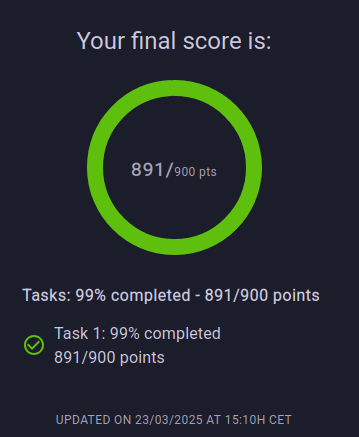
\includegraphics[width=0.3\textwidth]{challenge_result}
    \end{center}

    Back to this Project of Object Detection, I tried to use Yolo-11s on the images from the challenge I mentioned and a YouTube's video entirely of butterflies,
    the results are shown in the figure~\ref{fig:pre-trained}
    \begin{figure}
    \begin{subfigure}{.9\textwidth}
      \centering
      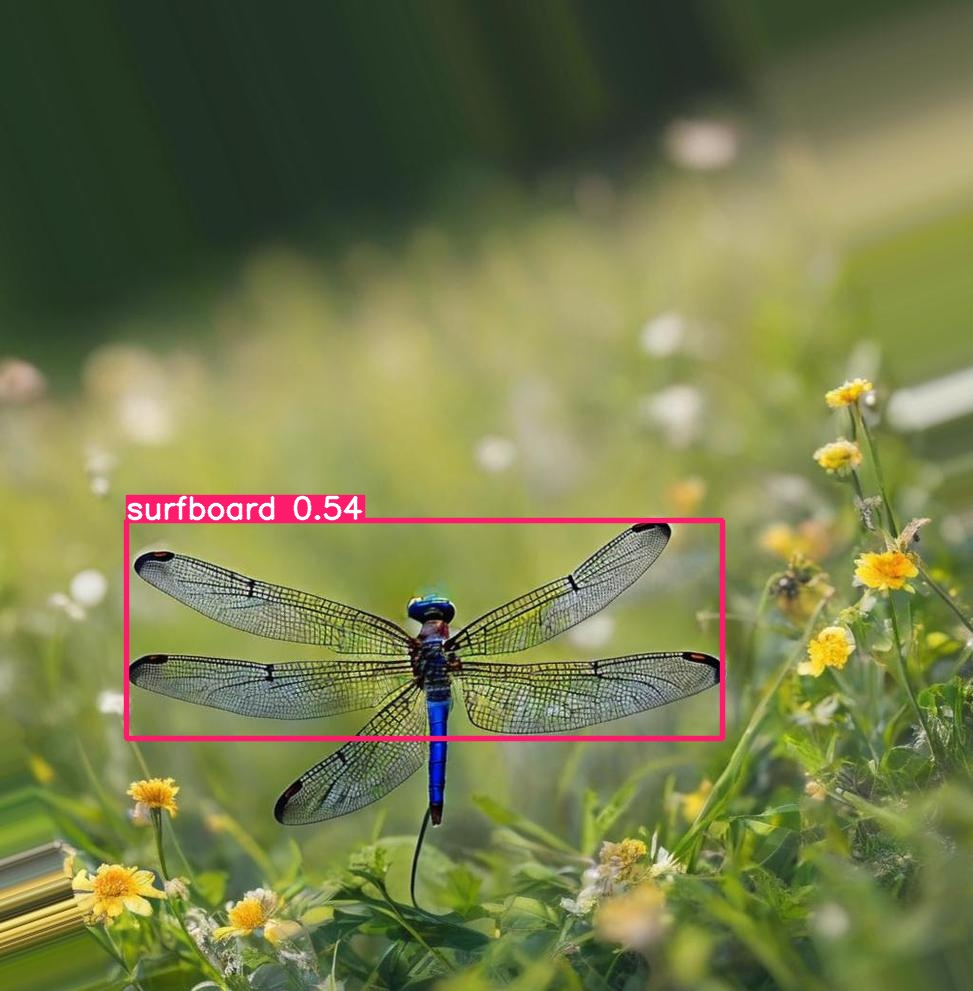
\includegraphics[width=.4\linewidth]{pretrained/negative_imagen_723}
      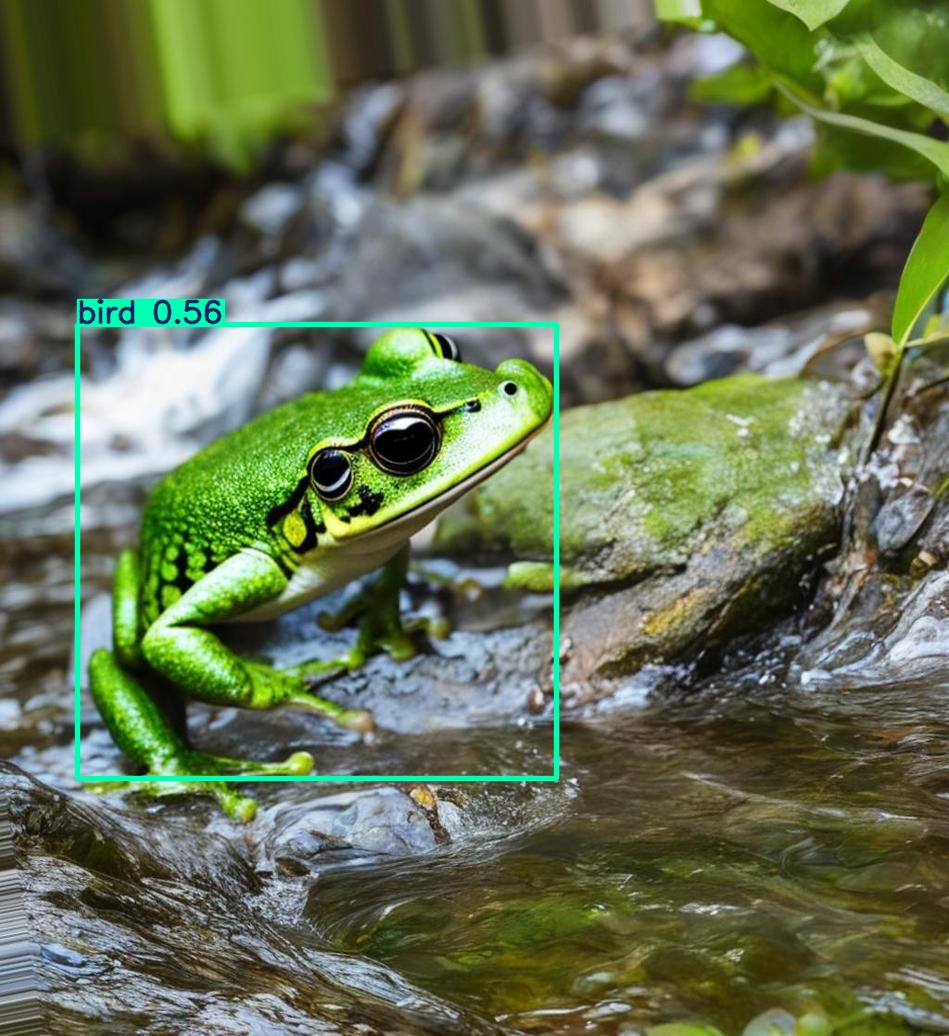
\includegraphics[width=.4\linewidth]{pretrained/negative_imagen_880}
      \caption{Negative class in the training data of the challenge}
      \label{fig:negative-pretrained}
    \end{subfigure}

    \begin{subfigure}{.9\textwidth}
      \centering
      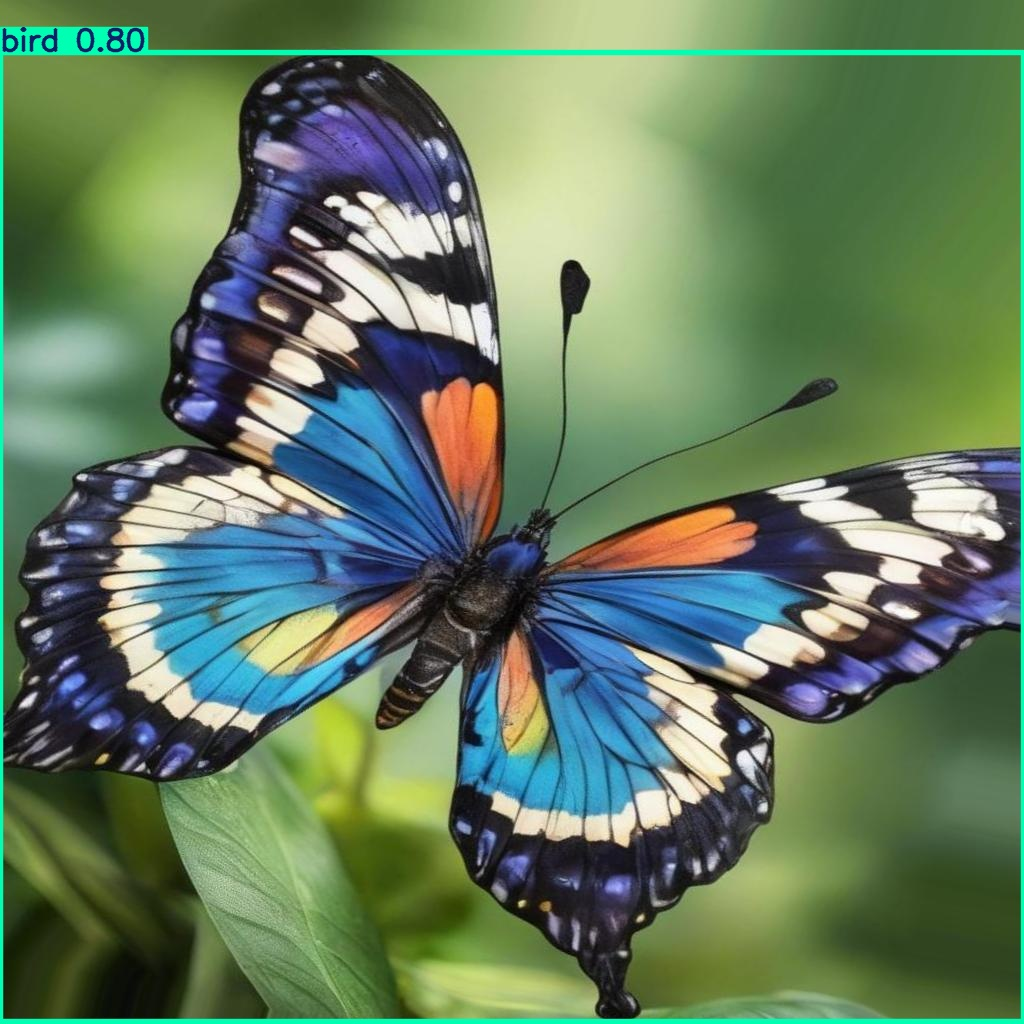
\includegraphics[width=.4\linewidth]{pretrained/positive_imagen_45}
      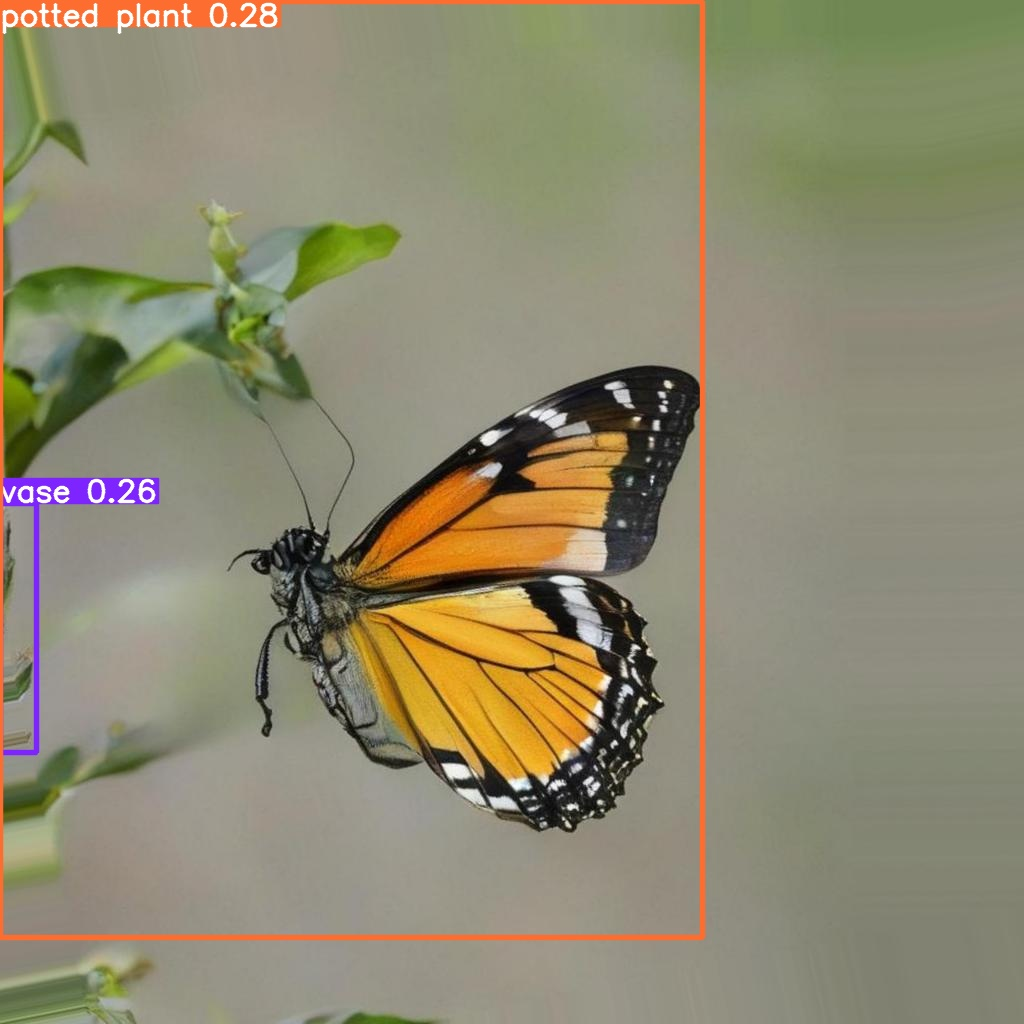
\includegraphics[width=.4\linewidth]{pretrained/positive_imagen_888}
      \caption{Positive class in the training data of the challenge}
      \label{fig:positive-pretrainied}
    \end{subfigure}

    \begin{subfigure}{.9\textwidth}
        \centering
        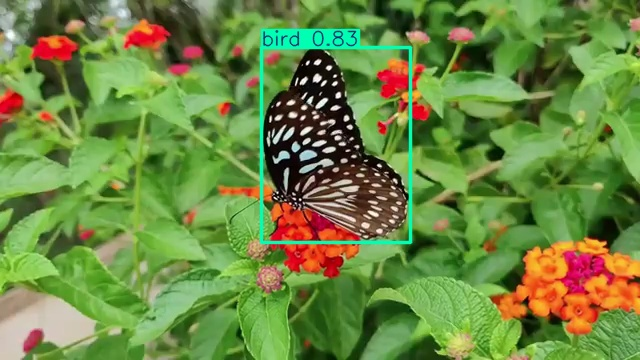
\includegraphics[width=.4\linewidth]{pretrained/photogram_16}
        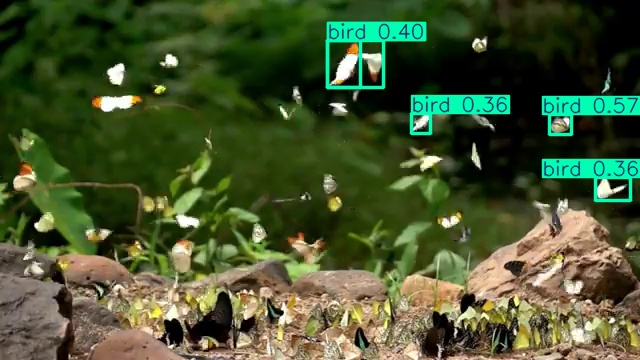
\includegraphics[width=.4\linewidth]{pretrained/photogram_93}
        \caption{Images of the YouTube video}
        \label{fig:video-pretrainied}
    \end{subfigure}
    \caption{Images results using only the pre-trained Yolo 11s}
    \label{fig:pre-trained}
    \end{figure}

    \newpage
    \centerline{\Large\textbf{Deep Learning Project 2: Object detection}}

\end{document}